\documentclass[10pt]{article}
\usepackage[a4paper, total={6in, 10in}]{geometry}
\usepackage{blindtext}
\usepackage{titling}
\usepackage{authblk}
\usepackage{graphicx}

\graphicspath{ {./img/} }

\predate{}
\postdate{}

\title{Accelerating Research with AWS IoT}
\author[1]{Marcilio Mendonca}
\author[1]{Bruno Vitali}
\author[1]{Arjun Shakdher}
\author[2]{Brent Maranzano}
\author[2]{Giuseppe Cogoni}
\author[2]{Bo Du}
\author[1]{Bryan Stone}
\author[1]{Don Bennett}

\affil[1]{AWS}
\affil[2]{Pfizer, Inc.}

\date{} % clear date
\begin{document}

\maketitle

\section*{}
Intro/Abstract here.


\section*{Background}
The speed of designing synthetic routes and defining 
formulations for new drug substances can be limited by the
rate at which the data becomes available for decision making. 
Much of the data is generated by offline laboratory
experiments, which requires process sampling, subdividing, 
transporting and consequently time-consuming sample 
preparation prior to analysis, in addition to the time
to analyze, interpret and report the results. An obvious
path to accelerate sample measurements is to increase the
number of analyses that can be performed in parallel by
either increasing the staff or through automation.
Alternatively, the entire process can be shortened by performing
the analysis in-situ. This approach, referred to as 
Process Analytical Technology (PAT), has been used in the
pharmaceutical industry for decades, but has been limited
to monitoring a few key parameters, most commonly using spectroscopic tools. 
The advent of miniature, cheap electronics coupled 
with the Internet of Things (IoT) has opened the possibility of 
monitoring a wide range of parameters in real-time.
The one obstacle that has inhibited the widespread adoption
of IoT in the pharmaceutical industry is the lack of a secure, 
scalable and cost-effective platform that can be used to store, 
analyze and visualize the data. In this paper, we describe the development of a
combination of on-premise and cloud-based IoT platform
that can be used to monitor and analyze data from a wide
range of sensors. The platform is designed to be scalable,
secure and cost-effective, and is demonstrated 
by monitoring the crystallization of a drug substance in real-time.

\section*{Architecture}
The key to a successful IoT platform is the ability to
scale to a large number of devices that can be readily implemented 
in various processes with minimal experience or training
by the end user e.g. “plug-n-play”. 
This minimal training interface often requires developing custom
in-house applications that make calibration, measurement
and analysis simple and robust. Moreover, the IoT platform 
must handle the large amount of data generated by
the sensors securely and cost-effectively. See Figure \ref{architecture}.

	\begin{figure}[h]
	\centering
	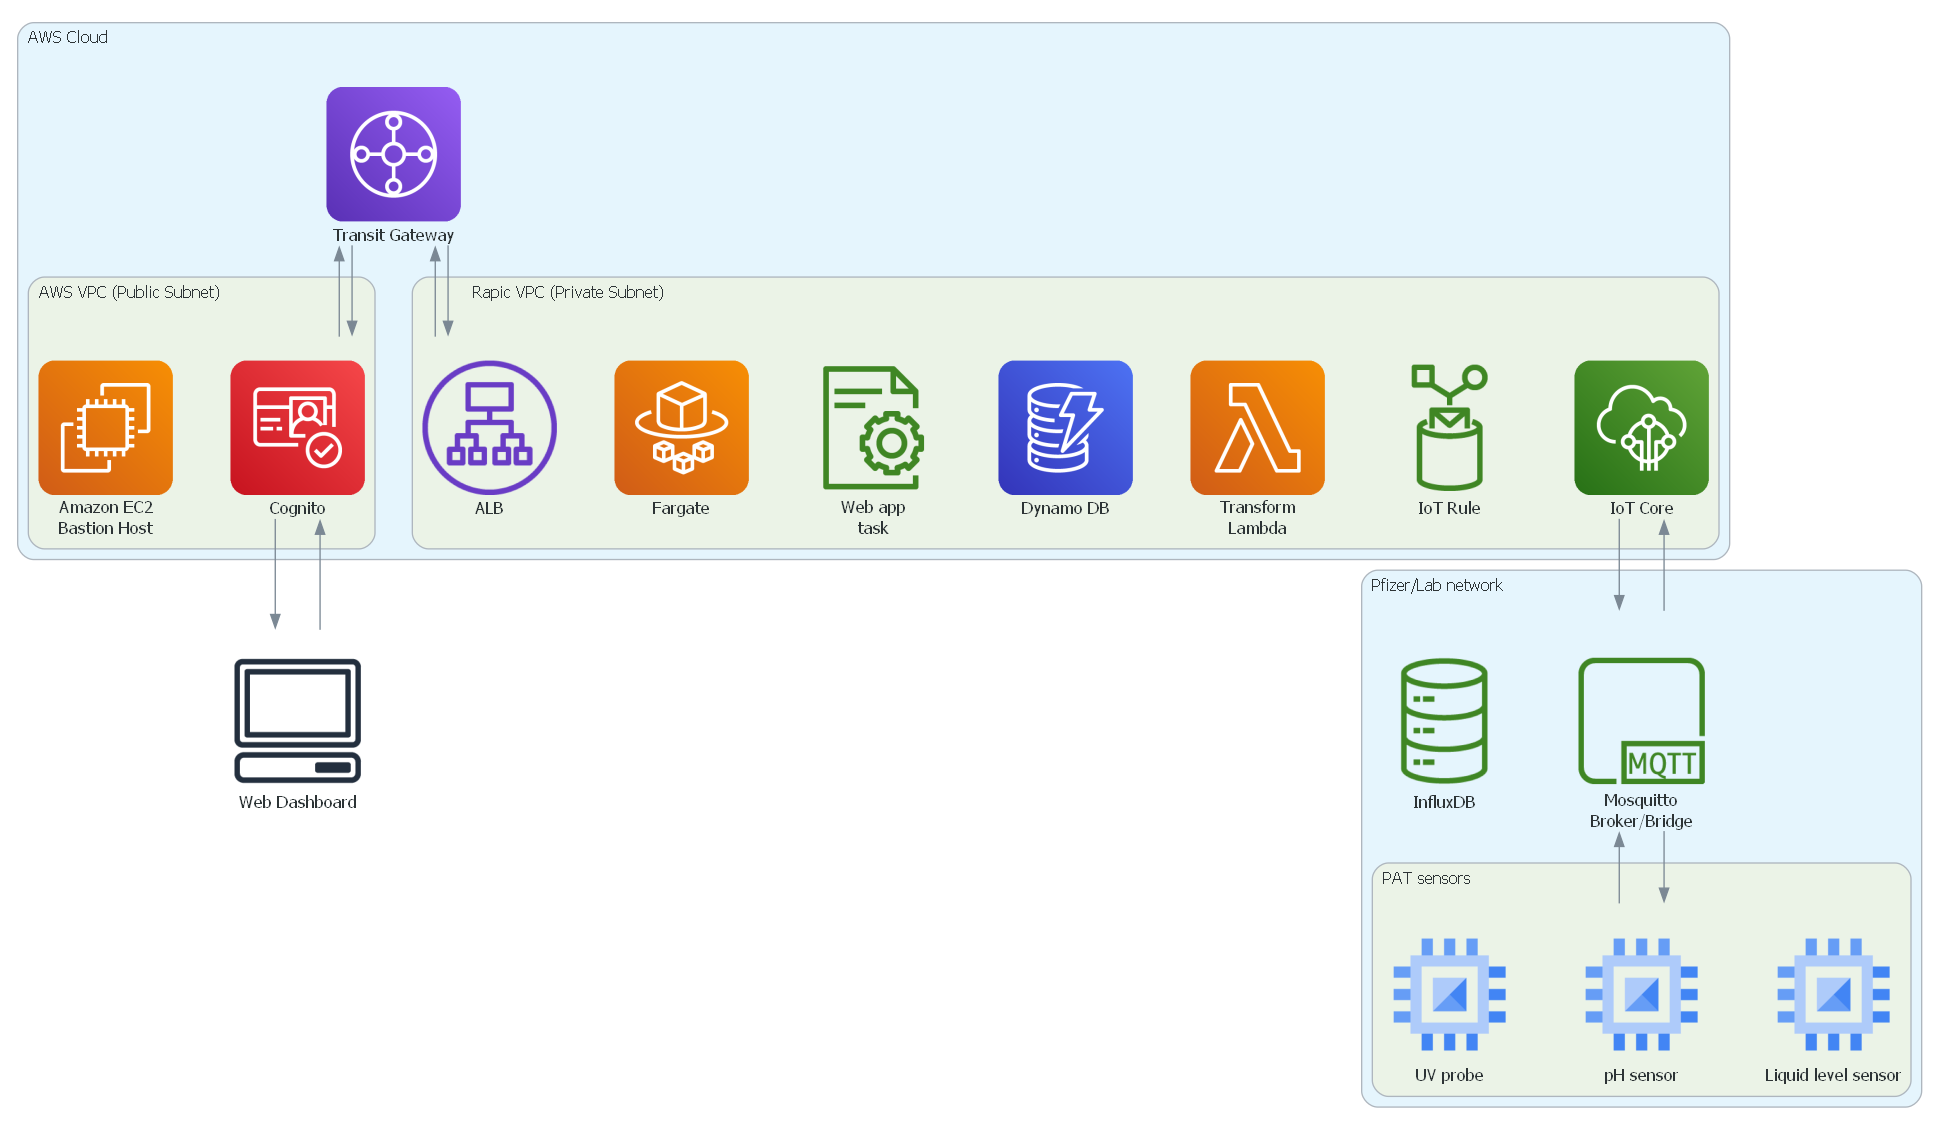
\includegraphics[width=0.5\textwidth]{architecture}
	\caption{Architecture IoT example}
	\label{architecture}
	\end{figure}

\section*{Interfacing the laboratory instruments}

\blindtext

\section*{Data visualization and instrument control}

\blindtext

\section*{Conclusions}

\blindtext


\end{document}